\section{Differential Power Analysis (DPA)}

\begin{frame}
    \frametitle{Differential Power Analysis }

    \textbf{Differential Power Analysis (DPA)} is a statistical method designed to identify data-dependent correlations in power measurements.

    The technique partitions sets of power traces into two subsets and computes the difference of the averages for those subsets.

    \begin{block}{Key Insight}
         If the subsets are \textbf{truly correlated} with secret-dependent power, their \textbf{average power traces will differ}.\newline If not, the difference between averages approaches zero as the number of traces increase.
    \end{block}

    This allows even very small correlations to be statistically isolated despite noise.
\end{frame}


\begin{frame}
    \frametitle{Detecting Leakage}

    By computing the difference between the average traces of the two subsets at each time point:

    \begin{itemize}
      \item Significant non-zero differences indicate a correlation with secret data.

      \item As the dataset grows, random noise averages out, revealing the leakage signal.

      \item This process can be automated across entire traces without prior knowledge of where leakage occurs.
    \end{itemize}
\end{frame}

\begin{frame}
    \frametitle{DPA: General Overview of the Algorithm}    
    \begin{enumerate}
        \item \textbf{Measure:} Capture a large number power traces with the victim device given a set of inputs.
        \item \textbf{Define a Selection Function:} A function that predicts a single bit of an intermediate value inside the cryptographic algorithm, based on a known value (like plaintext or ciphertext) and a \textit{guess} for a part of the key.
        
        \item \textbf{Partition Traces:} For a specific \textit{key guess}, classify all captured traces into two bins: one where the selection function predicts '0', and one where it predicts '1'.
        
        \item \textbf{Compare the Sets:} Calculate the average trace for each of the two sets. Then, compute the pointwise difference between these two average traces.
    \end{enumerate}
    \begin{block}{}
        \textbf{Key guess correct:} a "spike" will appear in the difference trace. \newline 
        \textbf{Key guess wrong:} partitioning is random, and the difference trace will be close to zero.
    \end{block}
\end{frame}


% Slide: Example: Visualizing DPA Averages and Differences
\begin{frame}
    \frametitle{Visualizing DPA Results: Case Study}

    

        \begin{itemize}
            \item The \textbf{top trace} is the average of all measured traces where the LSB was 1 (over the first two rounds of AES).
            \item The \textbf{second trace} is the average where the LSB was 0.
        \end{itemize}
        The two averages are visually very similar—differences due to leakage are much smaller than overall power consumption variations.

    % Place for figure inclusion
    \begin{figure}
        \centering
        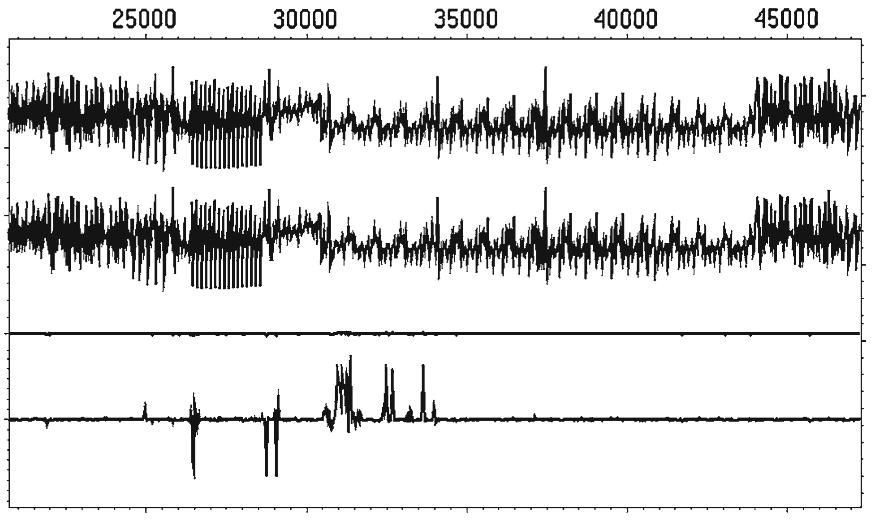
\includegraphics[width=0.60\textwidth]{main thing/Pictures/DPA_classic.png}
        \caption{Outcome of a DPA experiment against an AES smart card. The analysis targets the LSB of the first S-box output in the first round.}
    \end{figure}
\end{frame}


\begin{frame}
    \frametitle{Making Leakage Visible}

    \begin{itemize}
        \item The \textbf{third trace} in the figure shows the difference between the two subset averages. This line appears mostly flat, as the differences are small and masked by the y-axis scale.
        \item The \textbf{bottom trace} is the same difference but scaled up (e.g. $\times 15$), making the leakage spikes clearly visible.
    \end{itemize}

    \begin{block}{Leakage Interpretation}
        Spikes in the scaled difference trace correspond to moments when the targeted S-box output bit is manipulated inside the device. Spikes disappear after the first round, when the internal state is no longer correlated with the targeted bit.
    \end{block}

    High numbers of traces (e.g., 4,000) reduce noise, making the leakage clearer.
\end{frame}

% Slide: The Role of Selection Functions in DPA
\begin{frame}
    \frametitle{Selection Functions in Differential Power Analysis}

    The effectiveness of a DPA test critically depends on the choice of \textbf{selection function}.

    \begin{block}{Definition}
        A selection function is \textbf{used to assign traces to subsets} and is typically based on an educated guess as to a possible value for one or more intermediate values within a cryptographic calculation
    \end{block}
    Selection functions can be as simple as the predicted output bit of an S-box, or more complex, combining multiple bits or difference values.
    \begin{alertblock}{}
    \begin{itemize}
    \item If the final DPA trace shows \textbf{significant spikes}, the \textbf{selection function is correlated} with an internal value computed by the device.
        \item If not, the prediction is either \textbf{incorrect} or too weakly correlated to detect.
        \end{itemize}
    \end{alertblock}
\end{frame}


% Slide 1: DPA Targets the First Round of AES
\begin{frame}
    \frametitle{DPA Attack on AES-128: Overview}

    To illustrate the DPA process, we examine a classic attack on AES-128 encryption using real power traces from a smart card device. \newline
    \begin{block}{Quick memory refresher on AES}
        \begin{itemize}
            \item AES is a block cipher (symmetric)
            \item AES runs in multiple \textbf{rounds}; each round performs 4 operations
            \item AES takes blocks of 16 bytes as input and a key that is 16 (AES-128), 24 (AES-192) or 32 (AES-256) bytes long 
            \item Plaintext and ciphertext are always the same size
        \end{itemize}
    \end{block}
    We will attack the first round of AES.
\end{frame}

\begin{frame}{AES-128 Rounds}
     \begin{figure}
    
        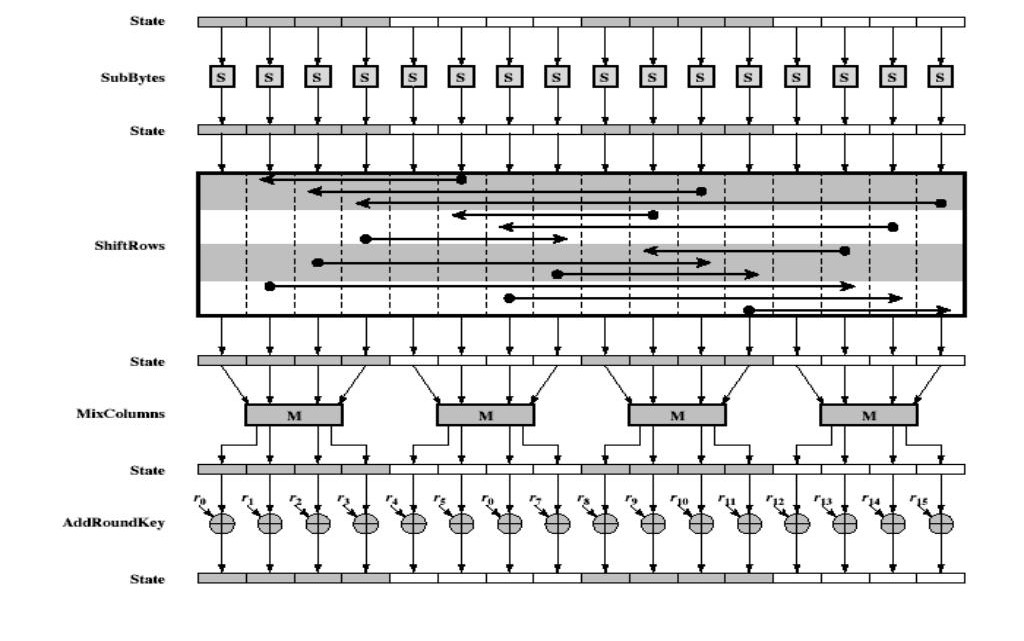
\includegraphics[width=1\textwidth]{main thing/Pictures/aes-round-l.jpg}
        
    \end{figure}
\end{frame}


\begin{frame}
    \frametitle{AES-128 Round 1: Steps and Target}

    The first round of AES-128 consists of these steps:
    \begin{enumerate}
        \item \textbf{Initialization:} State is set to the 16-byte plaintext.
        \item \textbf{AddRoundKey:} The 16-byte secret key is XORed with the state.
        \item \textbf{SubBytes:} Each state byte is substituted using the S-box.
        \item \textbf{ShiftRows:} Each row is cyclically shifted.
        \item \textbf{MixColumns:} Each column is mixed by a linear operation.
    \end{enumerate}

    \begin{figure}
        \centering
        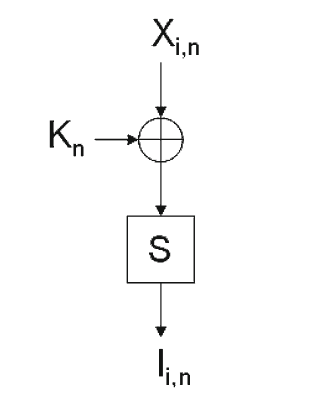
\includegraphics[width=0.25\textwidth]{main thing/Pictures/AddRoundKey_SBox_Diagram.png}
        \caption{The DPA attack focuses on the output of \textit{AddRoundKey} and \textit{SubBytes}, as shown in the figure.}
    \end{figure}
    
\end{frame}


\begin{frame}
    \frametitle{Intermediate Value \& Attack Notation}

    For each power trace $i$:
    \begin{itemize}
        \item $X_{i,n}$: The $n^{th}$ byte of plaintext in trace $i$ (known).
        \item $K_n$: The unknown $n^{th}$ byte of the round key (to be recovered).
        \item $I_{i,n}$: The $n^{th}$ byte of the state after SubBytes in round 1.
    \end{itemize}
    \begin{block}{}
    These terms are related:
    \[
        I_{i,n} = S[X_{i,n} \oplus K_n]
    \]
    where $S[\cdot]$ denotes the AES S-box.
    \end{block}
\end{frame}


\begin{frame}
    \frametitle{Key Search Strategy in DPA}

    Since $X_{i,n}$ is known, $K_n$ is unknown, and $S[\cdot]$ is public:

    \begin{itemize}
        \item For a candidate $K_n$, compute $I_{i,n}$ for each trace.
        \item Use a \textbf{selection function} (e.g., take the LSB of $I_{i,n}$) to assign each trace to subset 0 or 1.
        \item Repeat for all 256 possible values of $K_n$. Each round key requires only 256 guesses.
    \end{itemize}

\begin{block}{DPA Advantage}
        This divide-and-conquer method makes brute-force keyspace attack on AES feasible by turning a $2^{128}$ search into a succession of practical $2^8$ (256) searches. \newline
    DPA tests which candidate $K_n$ aligns with actual device leakage, byte by byte, to reveal the full 128-bit AES key.
    \end{block}
\end{frame}
% Slide 1: Subset 0
\begin{frame}
    \frametitle{Key Guess \textcolor{orange}{0x01} Binning Example}
    
    \centering
    \begin{tblr}{
        width = 0.8\linewidth,
        colspec = {Q[c,$]Q[c,$]Q[c,$]Q[c,$]Q[c,$]},
        row{1} = {cyan9, font=\bfseries},
        row{even} = {gray9},
        row{odd} = {white},
        hlines,
        vlines,
    }
        Input Data & Key Guess & XOR Output & S-Box Output & Subset \\
        \texttt{0xC7} & \texttt{0x01} & \texttt{0xC6} & \texttt{0xC7} & \textcolor{blue}{0} \\
        \texttt{0x1F} & \texttt{0x01} & \texttt{0x1E} & \texttt{0x1F} & \textcolor{blue}{0} \\
        \texttt{0x2C} & \texttt{0x01} & \texttt{0x2D} & \texttt{0x2C} & \textcolor{blue}{0} \\
        \texttt{0x89} & \texttt{0x01} & \texttt{0x88} & \texttt{0x89} & \textcolor{blue}{0} \\
        \texttt{0x01} & \texttt{0x01} & \texttt{0x00} & \texttt{0x01} & \textcolor{red}{\textbf{1}} \\
        \texttt{0xD2} & \texttt{0x01} & \texttt{0xD3} & \texttt{0xD2} & \textcolor{blue}{0} \\
    \end{tblr} \newline \newline
        \centering \textit{More traces are needed of course}
    
    
    
\end{frame}
% Slide 2: Subset 1
\begin{frame}
    \frametitle{Key Guess \textcolor{orange}{0x3D} Binning Example}
    
    \centering
    \begin{tblr}{
        width = 0.8\linewidth,
        colspec = {Q[c,$]Q[c,$]Q[c,$]Q[c,$]Q[c,$]},
        row{1} = {cyan9, font=\bfseries},
        row{even} = {gray9},
        row{odd} = {white},
        hlines,
        vlines,
    }
        Input Data & Key Guess & XOR Output & S-Box Output & Subset \\
        \texttt{0xC7} & \texttt{0x3D} & \texttt{0xFA} & \texttt{0x2D} & \textcolor{red}{1} \\
        \texttt{0x1F} & \texttt{0x3D} & \texttt{0x22} & \texttt{0x93} & \textcolor{red}{1} \\
        \texttt{0x2C} & \texttt{0x3D} & \texttt{0x11} & \texttt{0x82} & \textcolor{blue}{0} \\
        \texttt{0x89} & \texttt{0x3D} & \texttt{0xB4} & \texttt{0x8D} & \textcolor{red}{1} \\
        \texttt{0x01} & \texttt{0x3D} & \texttt{0x3C} & \texttt{0xEB} & \textcolor{red}{\textbf{1}} \\
        \texttt{0xD2} & \texttt{0x3D} & \texttt{0xEF} & \texttt{0xDF} & \textcolor{red}{1} \\
    \end{tblr}\newline \newline
        \centering \textit{More traces are needed of course}

    
\end{frame}


% Slide 1: Interpreting Difference of Subset Averages
\begin{frame}
    \frametitle{Interpreting Differences of Averages in DPA}

    After partitioning traces using a selection function, the difference of subset averages is examined:

    \begin{block}{Key Insight}
        If the predicted S-box output bit correlates with the power measurements, large spikes appear in the differential trace for the correct key guess.
    \end{block}

    For incorrect guesses, the predicted values are unrelated to the device data, yielding little to no significant spike.
\end{frame}

% Slide 2: AES Key Byte Guessing: Example Results
\begin{frame}
    \frametitle{DPA Difference Traces for AES Key Byte Candidates}

    Differential traces were computed for all possible values of the first round key byte $K_0$ (0 to 255).

    \begin{itemize}
        \item The figure shows traces for guesses $K_0 = 101$ to $105$.
        \item The correct key byte $K_0=103$ is identified by strong spikes in the differential trace.
        \item Incorrect guesses produce smaller spikes or flat traces.
    \end{itemize}

    \begin{figure}
        \centering
        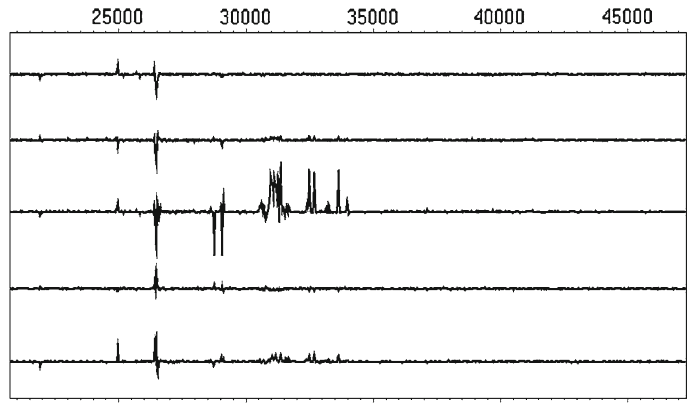
\includegraphics[width=0.65\textwidth]{main thing/Pictures/DPA_diff_trace.png}
    \end{figure}
\end{frame}

\begin{frame}
    \frametitle{Completing the Key Recovery}

    This analysis can be iterated independently for each of the 16 bytes ($n = 0, \ldots, 15$) of the AES state.

    \begin{block}{Important Note}
        The same set of traces can be reused for each round key since each attack tests different hypotheses.
    \end{block}

    This divide-and-conquer approach enables full recovery of the 128-bit AES key.
\end{frame}

\begin{frame}
    \frametitle{Mathematical Formulation of DPA}

    Let:
    \begin{itemize}
        \item $T = \{T_i\}_{i=1}^m$ be the set of collected power traces,
        \item $T_i[j]$ be the power measurement at the $j^\text{th}$ time sample in trace $i$,
        \item $C = \{C_i\}_{i=1}^m$ be the set of known inputs or outputs corresponding to each trace,
        \item $D(C_i, K_n)$ be a binary selection function dependent on known data $C_i$ and a key guess $K_n$.
    \end{itemize}

    Then, the differential trace $\Delta D[j]$ at time offset $j$ for key guess $K_n$ is computed as:

    \[
        \Delta D[j] = 
        \frac{
            \sum_{i=1}^m D(C_i, K_n) \cdot T_i[j]
        }{
            \sum_{i=1}^m D(C_i, K_n)
        }
        -
        \frac{
            \sum_{i=1}^m (1 - D(C_i, K_n)) \cdot T_i[j]
        }{
            \sum_{i=1}^m (1 - D(C_i, K_n))
        }
    \]

    This difference highlights points in time where the power consumption correlates with the selection function’s prediction, helping identify the correct key guess.
\end{frame}


\begin{frame}
    \frametitle{Extending DPA Across Modes and Devices}

    DPA can be adapted for different cipher modes or hardware.

    For example, the figure in the next slide shows a DPA attack on an AES-CBC implementation in an FPGA:

    \begin{itemize}
        \item The ciphertext is available instead of plaintext; so the selection function targets last round key bytes.
        \item A single oscilloscope trace capturing all AES operations is split into many operations for analysis.
    \end{itemize}
\end{frame}

\begin{frame}{Extending DPA Across Modes and Devices}
    \begin{figure}
        \centering
        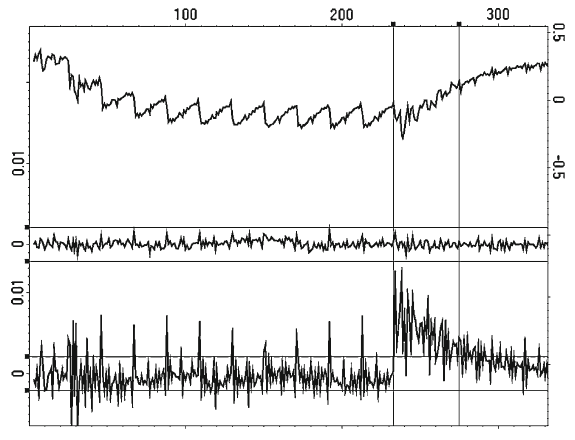
\includegraphics[width=0.75\textwidth]{main thing/Pictures/aes_cbc_fpga.png}
        \caption{DPA results against AES-CBC on FPGA; top: average trace, middle: incorrect key guess, bottom: correct key guess.}
    \end{figure}
\end{frame}







